chapter{Anforderungsspezifikation}

\section{Einf"uhrung}

\subsection{Zweck}
Dieses Kapitel legt die Anforderungen an das Programm \textsc{NetBomb} fest.

\subsection{G"ultigkeitsbereich}
Semesterarbeit Software Engineering, Sommersemester 2002

\subsection{Definitionen, Akronyme, Abk"urzungen}
Siehe Anhang \ref{glossar} auf Seite \pageref{glossar}.

\section{Allgemeine Beschreibung}
\subsection{Spielregeln}

Ziel des Spiels ist es, die gegnerische Spielfigur mittels einer Bombe und dessen Bombenstrahl zu eliminieren.
Im Spiel gibt es zwei Spielfiguren, eine fixe Anzahl Mauern und eine variable Anzahl W"ande.
Die Spielfigur kann W"ande sprengen, Mauern sind unzerst"orbar.
Die Spielfigur kann weder durch W"ande noch durch Mauern gehen.
Unter gesprengten W"anden k"onnen sich Bomben oder Feuersymbole befinden. Das Aufheben einer Bombe erlaubt der Spielfigur
das Legen einer zus"atzlichen Bombe in Serie. Das Aufheben einer Flamme erlaubt der Spielfigur einen um ein Feld
l"angerer Bombenstrahl.
Die zwei Spielfiguren sind gegenseitig transparent. Sie k"onnen sich kreuzen.

\begin{figure}[H]
  \begin{center}
    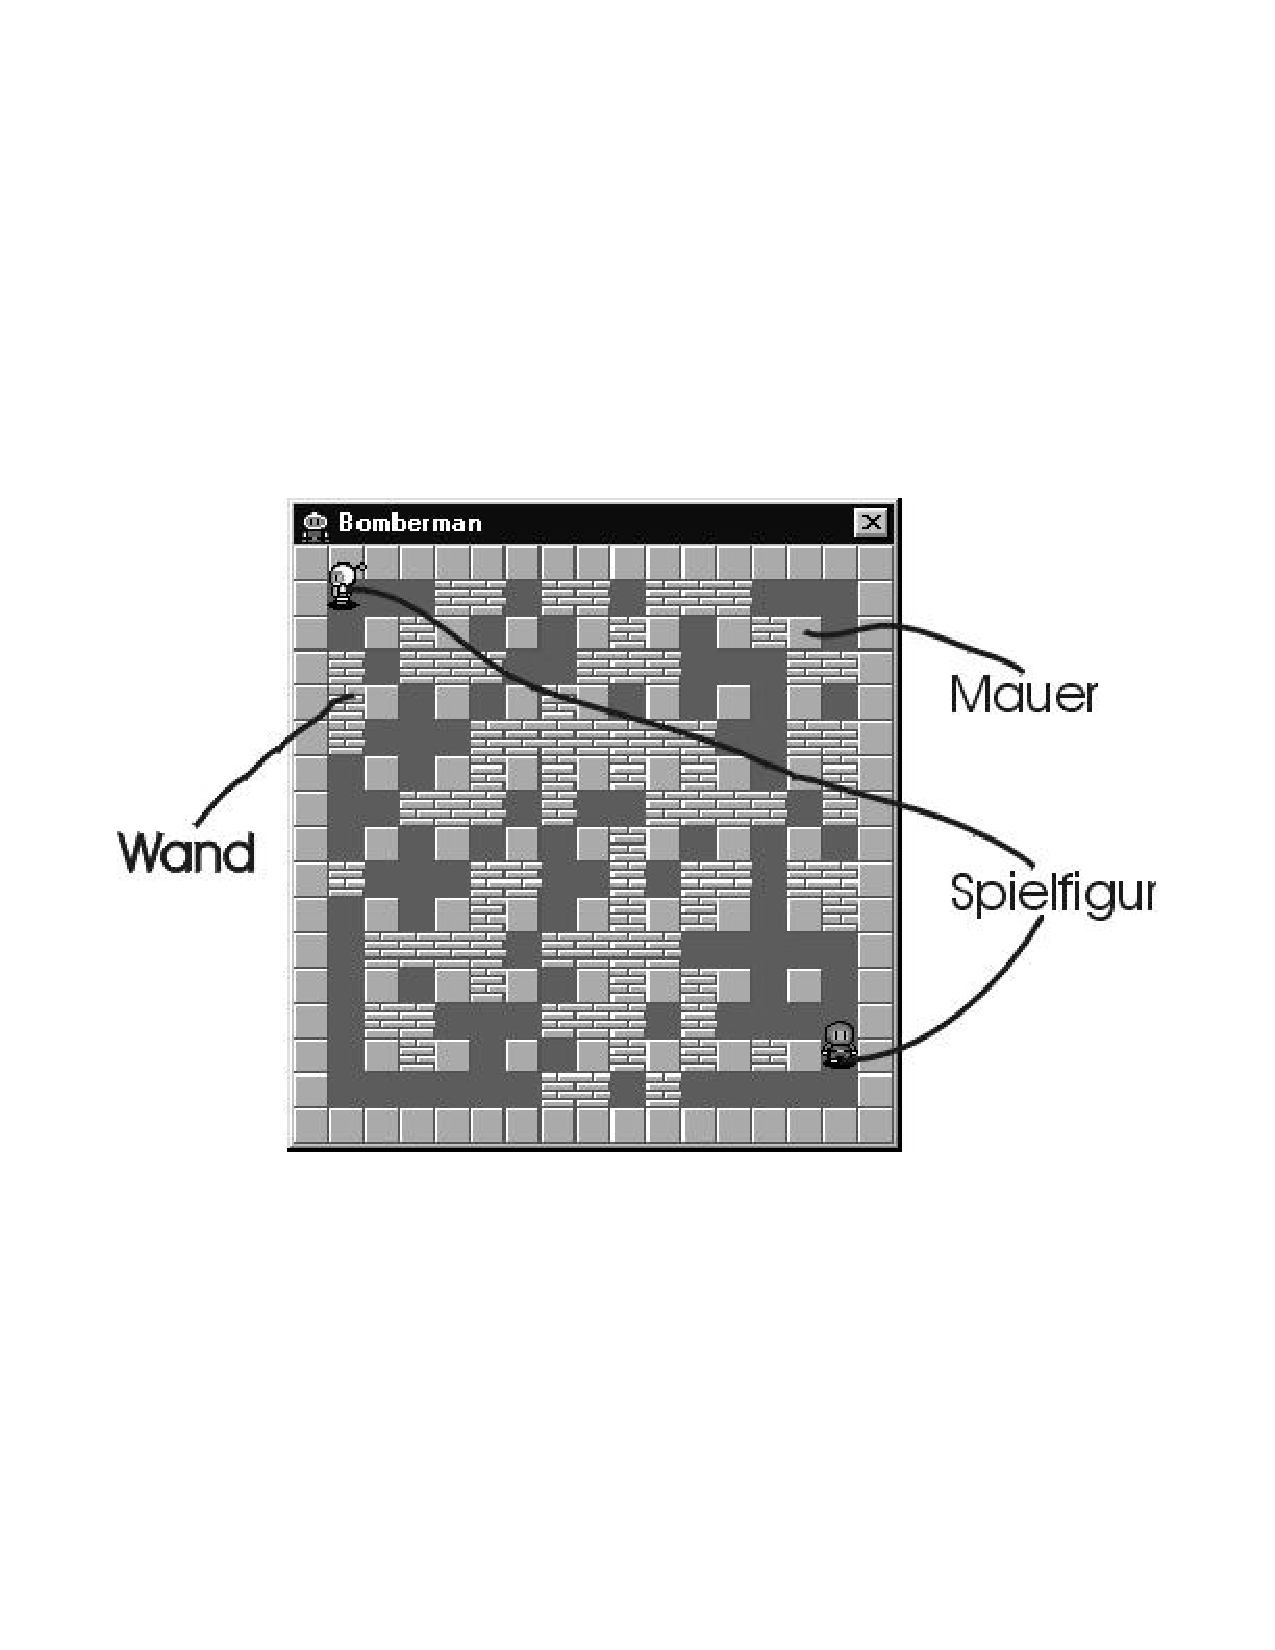
\includegraphics[width=10cm]{./images/bomber.pdf} \\
  \end{center}
  \caption{Bomberman Spiel}
\end{figure}

\subsection{Benutzergruppen}
Alle Menschen ob jung oder alt, weiblich oder m"annlich, die Freude an Computerspielen haben.

\subsection{M"ogliche Erweiterungen}
\begin{itemize}
\item Sound Unterst"utzung
\item spezielle Powerup-Icons, die von der Spielfigur aufgenommen werden k"onnen.
\item Highscore Anzeige
\end{itemize}

\subsection{Zu erwartende Probleme}
wurden bereits im Dokument Projektplan eingetragen.

\subsection{Annahmen}
Da die von uns verwendeten Technologien f"ur uns neu sind, sind wir uns bewusst, dass das Risiko vorhanden ist, dass wir
die Anforderungen nicht vollst"andig erf"ullen k"onnen. Dieses Dokument wurde in der Annahme geschrieben, dass wir die
auftretenden Probleme l"osen k"onnen. Ansonsten werden wir die Anforderungen zusammen mit dem Betreuer anpassen.

\subsection{Abh"angikeiten}
Funktionalit"at Qt-Bibliothek und KDE-Bibliothek.

\section{Anforderungen im Einzelnen}

\subsection{Funktionale Anforderungen Iteration 1}


\begin{table}[H]
  \begin{center}
    \begin{tabular}{|p{20mm}| p{85mm}| p{20mm}|}
    \multicolumn{3}{l}{\textbf{Spiel}} \\
    \hline Referenz & Funktion & Priorit"at \\
    \hline A1.1 & Spiel starten & 1 \\
    \hline A1.2 & Spiel beenden & 1 \\
    \hline A1.3 & Spielregeln "uberwachen & 1 \\
    \hline
    \end{tabular}
  \end{center}
  \caption{Spiel Funktionen Iteration 1}
\end{table}

\begin{table}[H]
  \begin{center}
    \begin{tabular}{|p{20mm}|p{85mm}|p{20mm}|}
    \multicolumn{3}{l}{\textbf{Spielfigur}} \\
    \hline Referenz & Funktion & Priorit"at \\
    \hline A2.1 & Figur bewegen & 1 \\
    \hline
    \end{tabular}
  \end{center}
  \caption{Spielfigur Funktionen Iteration 1}
\end{table}


\begin{table}[H]
  \begin{center}
    \begin{tabular}{|p{20mm}|p{85mm}|p{20mm}|}
    \multicolumn{3}{l}{\textbf{Spielfeld}} \\
    \hline Referenz & Funktion & Priorit"at \\
    \hline A3.1 & Hintergrund zeichnen & 1 \\
    \hline A3.2 & Mauern und W"ande zeichnen & 1 \\
    \hline A3.3 & Spielfigur zeichnen & 1 \\
    \hline
    \end{tabular}
  \end{center}
  \caption{Spielfeld Funktionen Iteration 1}
\end{table}


\subsection{Funktionale Anforderungen Ieration 2}


\begin{table}[H]
  \begin{center}
    \begin{tabular}{|p{20mm}|p{85mm}|p{20mm}|}
    \multicolumn{3}{l}{\textbf{Spiel}} \\
    \hline Referenz & Funktion & Priorit"at \\
    \hline A1.4 & Spielstand aktualisieren & 2 \\
    \hline A1.5 & Highscore speichern & 2 \\
    \hline
    \end{tabular}
  \end{center}
  \caption{Funktionen Spiel Iteration 2}
\end{table}



\begin{table}[H]
  \begin{center}
    \begin{tabular}{|p{20mm}|p{85mm}|p{20mm}|}
    \multicolumn{3}{l}{\textbf{Spielfigur}} \\
    \hline Referenz & Funktion & Priorit"at \\
    \hline A2.2 & Bombe legen  & 2 \\
    \hline A2.3 & sterben      & 2 \\
    \hline
    \end{tabular}
  \end{center}
  \caption{Funktionen Spielfigur Iteration 2}
\end{table}



\begin{table}[H]
  \begin{center}
    \begin{tabular}{|p{20mm}|p{85mm}|p{20mm}|}
    \multicolumn{3}{l}{\textbf{Spielfeld}} \\
    \hline Referenz & Funktion & Priorit"at \\
    \hline A3.4 & Wand entfernen & 2 \\
    \hline
    \end{tabular}
  \end{center}
  \caption{Funktionen Spielfeld Iteration 2}
\end{table}



\begin{table}[H]
  \begin{center}
    \begin{tabular}{|p{20mm}|p{85mm}|p{20mm}|}
    \multicolumn{3}{l}{\textbf{Bombe}} \\
    \hline Referenz & Funktion & Priorit"at \\
    \hline A4.1 & explodieren & 2 \\
    \hline A4.2 & Reichweite berechnen & 2 \\
    \hline
    \end{tabular}
  \end{center}
  \caption{Funktionen Bombe Iteration 2}
\end{table}



\begin{table}[H]
  \begin{center}
    \begin{tabular}{|p{20mm}|p{85mm}|p{20mm}|}
    \multicolumn{3}{l}{\textbf{Netzwerk}} \\
    \hline Referenz & Funktion & Priorit"at \\
    \hline A5.1 & Server starten & 2 \\
    \hline A5.2 & Client anmelden & 2 \\
    \hline A5.3 & Spielelement Position "ubermitteln & 2 \\
    \hline A5.4 & Spielsituation synchronisieren & 2 \\
    \hline
    \end{tabular}
  \end{center}
  \caption{Funktionen Netzwerk Iteration 2}
\end{table}

%Use Cases
\subsection{Use Cases Iteration 1}
\subsubsection{UC01 Spiel starten}

\begin{table}[H]
  \begin{center}
    \begin{tabular}{|p{40mm}|p{90mm}|}
    \hline Ausl"osender Aktor & Spieler  \\
    \hline Zweck / Ziel & Spielfeld und Spielelemente zeichnen, Netzwerkverbindung aufbauen  \\
    \hline Priorit"at & 1 \\
    \hline Style & fully dressed \\
    \hline Anforderungen &  A1.1, A1.2, A3.1, A3.2, A3.3\\
    \hline Vorbedingung & - \\
    \hline Nachbedingung & Spielfeld und Spielelemente gezeichnet, Netzwerkverbindung aufgebaut. \\
    \hline Bemerkungen & - \\
    \hline
    \end{tabular}
  \end{center}
  \caption{UC01 Spiel starten}
\end{table}


\begin{center}
  \begin{tabular}{p{65mm} p{65mm}}
  \multicolumn{2}{l}{\textbf{Grundlegender Ablauf}} \\
  & \\
  \textbf{Aktor} & \textbf{System} \\
  1. Benutzer startet neues Spiel &  \\
  &  2. Leveldaten einlesen  \\
  &  3. Spielfeld zeichnen \\
  &  4. Spielelemente zeichnen \\
  &  5. wartet auf Benutzereingabe\\
  \multicolumn{2}{l}{\textbf{Erweiterungen}} \\
  \(\ast\)a zu jeder Zeit kann der Spieler das Spiel beenden & \\
  \end{tabular}
\end{center}


\subsubsection{UC02 Spielfigur bewegen}

\begin{table}[H]
  \begin{center}
    \begin{tabular}{|p{40mm}|p{90mm}|}
    \hline Ausl"osender Aktor & Spieler \\
    \hline Zweck / Ziel & Aktor kann Spielfigur in horizontaler oder vertikaler Richtung bewegen \\
    \hline Priorit"at & 1\\
    \hline Style & fully dressed \\
    \hline Zu erf"ullende Anforderungen & A1.3, A2.1, A3.3 \\
    \hline Vorbedingungen & UC01 \\
    \hline Nachbedingungen & Die Spielfigur wurde um ein Feld verschoben.\\
    \hline Bemerkungen & Dieser UC kann 1 oder n mal ausgef"uhrt werden. \\
    \hline
    \end{tabular}
  \end{center}
  \caption{UC02 Spielfigur bewegen}
\end{table}


\begin{center}
  \begin{tabular}{p{65mm} p{65mm}}
  \multicolumn{2}{l}{\textbf{Grundlegender Ablauf}} \\
  & \\
  \textbf{Aktor} & \textbf{System} \\
  1. Der Aktor verschiebt die Spielfigur um ein Feld nach links, rechts, oben oder unten. & \\
  & 2. zeichnet die Figur auf dem neuen Feld, sofern das Zielfeld nicht einer Wand oder einer Mauer enstpricht. \\
  \end{tabular}
\end{center}



\subsection{Optional}


\begin{table}[H]
  \begin{center}
    \begin{tabular}{|p{20mm}|p{85mm}|p{20mm}|}
    \multicolumn{3}{l}{\textbf{Spiel}} \\
    \hline Referenz & Funktion & Priorit"at \\
    \hline A1.6 & Spiel pausieren & 3 \\
    \hline A1.7 & Soundeffekte abspielen & 3 \\
    \hline A1.8 & Musik abspielen & 3 \\
    \hline
    \end{tabular}
  \end{center}
  \caption{optionale Funktionen Spiel}
\end{table}



\begin{table}[H]
  \begin{center}
    \begin{tabular}{|p{20mm}|p{85mm}|p{20mm}|}
    \multicolumn{3}{l}{\textbf{Spielfigur}} \\
    \hline Referenz & Funktion & Priorit"at \\
    \hline A2.4 & Bombe-Powerup aufnehmen & 3 \\
    \hline A2.5 & Flamme-Powerup aufnehmen & 3 \\
    \hline
    \end{tabular}
  \end{center}
  \caption{optionale Funktionen Spielfigur}
\end{table}


\begin{table}[H]
  \begin{center}
    \begin{tabular}{|p{20mm}|p{85mm}|p{20mm}|}
    \multicolumn{3}{l}{\textbf{Spieloptionen}} \\
    \hline Referenz & Funktion & Priorit"at \\
    \hline A6.1 & Sound ein/aus & 3 \\
    \hline A6.2 & Highscores anzeigen & 3 \\
    \hline A6.3 & Spielername eingeben & 3 \\
    \hline
    \end{tabular}
  \end{center}
  \caption{Spieloptionen}
\end{table}


\subsection{Leistungs- und Mengenanforderungen}
\label{LeistungsAnforderungen}
\subsubsection{Leistungsanforderungen}
Um die Spielbarkeit "ubers Netzwerk zu gew"ahrleisten, muss der Spielstatus von allen Spielern mindestens
alle 150ms synchronisiert werden.

\subsubsection{Mengenanforderungen}
Keine.

\subsection{Anforderungen an Schnittstellen}

\subsubsection{Benutzerschnittstelle}
Das System ist mit dem Keyboard und der Maus bedienbar.

\subsubsection{Software Schnittstellen}
Qt, KDE-Library

\subsection{Randbedingungen f"ur den Entwurf}

\subsubsection{"Ubereinstimmungen mit Normen}
SE01/02

\subsubsection{Einschr"ankungen bez"uglich Software}
Lauff"ahig unter KDE 2.2

\subsubsection{Einschr"ankungen bez"uglich Hardware}
Lauff"ahig unter allen UNIX-Derivaten, die KDE unterst"utzen. Die Leistungsanforderungen gelten f"ur ein Netzwerk (mind. 10Mb/s)
ohne zus"atzlichen Datenverkehr.

\subsection{Merkmale}

\subsubsection{Benutzbarkeit}
Die Bedienung des Programms entspricht den g"angigen KDE-Programmen:\\
\href{http://developer.kde.org/documentation/standards/kde/style/basics/index.html}{http://developer.kde.org/documentation/standards/kde/style/basics/index.html}

\subsection{Andere Anforderungen}

\subsubsection{Inbetriebnahme / Installation}
Standardinstallationsweg eines Linux-Quellcodes (configure, make, make install)

\subsubsection{Konfigurierbarkeit}
Alle Konfigurationen werden gespeichert. Die IP-Adresse des Spielservers kann eingegeben werden.
Optional kann der Spielername eingegeben werden.





